\documentclass[conference]{IEEEtran}
\IEEEoverridecommandlockouts
% The preceding line is only needed to identify funding in the first footnote. If that is unneeded, please comment it out.
\usepackage{cite}
\usepackage{amsmath,amssymb,amsfonts}
\usepackage{graphicx}
\usepackage{textcomp}
\usepackage{xcolor}
\def\BibTeX{{\rm B\kern-.05em{\sc i\kern-.025em b}\kern-.08em
    T\kern-.1667em\lower.7ex\hbox{E}\kern-.125emX}}
\title{
\begin{center}
\includegraphics[width=0.2\textwidth, left]{logoIITH.png}
\end{center}
\vspace{1cm}
{Distributive Law of Boolean Algebra}
}
\author{Meer Tabres Ali and G V V Sharma}
\begin{document}
\maketitle
\section{ABSTRACT}
Distributive law of Boolean Algebra is expressed by “ X.(Y+Z) = X.Y + X.Z ”. In this program, Two LEDs are used for checking the output. The outputs of both RHS and LHS parts must be same with random inputs.
\subsection{Logic Gates configuration}
Logic Gates configuration is shown in figure 1. 
\begin{figure}[h]
\centering
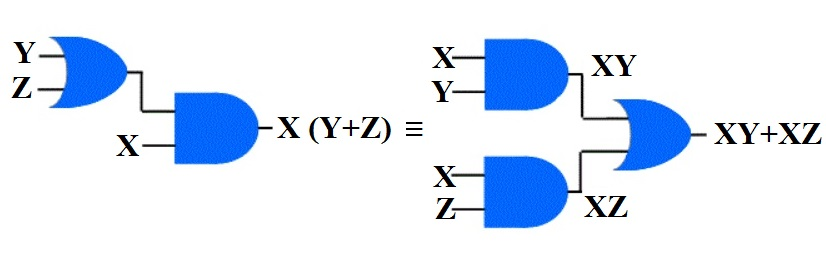
\includegraphics[width=0.4\textwidth]{Gates.jpg}
\caption{\label{fig:Gates}This frog was uploaded via the file-tree menu.}
\end{figure}
\subsection{Truth Table for Distributive Law}
Truth Table for Distributive Law is given in Table 1.
\begin{table}[htbp]
    \centering
\begin{tabular}{ | c | c | c | c | c | c | c | c | } \hline
X & Y & Z & Y+Z & X(Y+Z) & XY & XZ & XY+XZ \\\hline
0 & 0 & 0 & 0 & 0 & 0 & 0 & 0 \\
0 & 0 & 1 & 0 & 0 & 0 & 0 & 0 \\
0 & 1 & 0 & 0 & 0 & 0 & 0 & 0 \\
0 & 1 & 1 & 0 & 0 & 0 & 0 & 0 \\
1 & 0 & 0 & 0 & 0 & 0 & 0 & 0 \\
1 & 0 & 1 & 1 & 1 & 0 & 1 & 1 \\
1 & 1 & 0 & 1 & 1 & 1 & 0 & 1 \\
1 & 1 & 1 & 1 & 1 & 1 & 1 & 1 \\ \hline
\end{tabular}
\caption{\label{tab:widgets}Truth Table for Distributive Law}
\end{table}
\section{COMPONENTS}
Required components list has been given in Table 2
\begin{table}
\centering
\begin{tabular}{| c | c | c |} \hline
Components & Value & Quantity \\\hline
Resistors & 220 ohm & 2 \\
LEDs &  & 2 \\
Arduino & UNO & 1 \\
Jumper Wires &  & 20 \\
Breadboard & & 1 \\ 
\hline
\end{tabular}
\caption{\label{tab:widgets}Components}
\end{table}
\section{HARDWARE}
Make the connections between Arduino and LEDs as per the Table 3 and Figure 3.
\begin{table}
\begin{tabular}{|c | c | c | c | c | c |} \hline
 & \textbf{INPUT} & \textbf{INPUT} & \textbf{INPUT} & \textbf{OUTPUT} & \textbf{OUTPUT} \\\hline
 & X & Y & Z & X(Y+Z) & XY+XZ \\ \hline
Arduino & 2 & 3 & 4 & 5 & 6 \\ 
LEDs &  &  &  & LED1 & LED2 \\ \hline
\end{tabular}
\caption{\label{tab:widgets}}
\end{table}

\begin{figure}[h]
\centering
\includegraphics[width=0.4\textwidth]{LED.jpg}
\caption{\label{fig:LED}Connections between Arduino and LEDs.}
\end{figure}
\section{SOFTWARE}
1. Download the codes given in the link below and execute them.
2. Apply the inputs X, Y, and Z (either HIGH or LOW) to the Digital Pin no.s 2, 3 and 4 of Arduino as per the Truth table (Table 1).
\section{FINDINGS}
After the execution of codes, for different input variables (X, Y and Z), the output pins (5 and 6) of Arduino will be at the same level (both output pins will be at either HIGH or LOW simultaneously), and it causes both LEDs either to glow or off.
\section{CONCLUSION}
1. Distributive law is expressed by “X(Y+Z)=XY+XZ”, and here LHS = X(Y+Z), RHS = XY+XZ.
2. Codes are written for Distributive law and are executed. 
3. Result has been displayed on Two LEDs (i.e. LED1 and LED2). 
4. LED1 is assigned for LHS of the Boolean expression of Distributive Law.
5. LED2 is assigned for RHS of the Boolean expression of Distributive Law.
6. For random digital inputs X, Y and Z as per Truth table (at Arduino digital pins 2, 3 and 4), it has been noticed that the output pins (5 and 6) of Arduino are at the same level.
\end{document}